\subsubsection{pr03}
\label{subsubsec:pr03}
The obtained results were the following:
{
\renewcommand{\arraystretch}{2}
\begin{longtable}[h]{| c | c | c | c | c |}
    \hline
    \textbf{Failures} & \multicolumn{3}{c}{Time limit} & \\
    \hline
    \textbf{Search strategy} & \textbf{\textit{30 sec}} & \textbf{\textit{1 min}} & \textbf{\textit{2 min}} & \textbf{\textit{5 min}} \\
    \hline
    \endhead
    default search                                         &  4.405 &  6.511 & 14.998 &  61.397 \\
    \hline
    domWdeg, random                                        &  2.196 &  6.408 & 12.741 &  59.614 \\
    \hline
    domWdeg, random, Luby restart L=250                    &   233 &   351 &  8.464 &  51.010 \\
    \hline
    \textit{domWdeg, random, Luby restart L=250, LNS 85\%} &   106 &   107 &   178 &    223 \\
    \hline
    domWdeg, random, Luby restart L=250, LNS 15\%          &   616 &   624 &  3.265 &  64.619 \\
    \hline
    first fail, min                                        &  2.123 &  4.228 & 10.772 &  88.969 \\
    \hline
\end{longtable}
}
\begin{figure}[H]
    \centering
    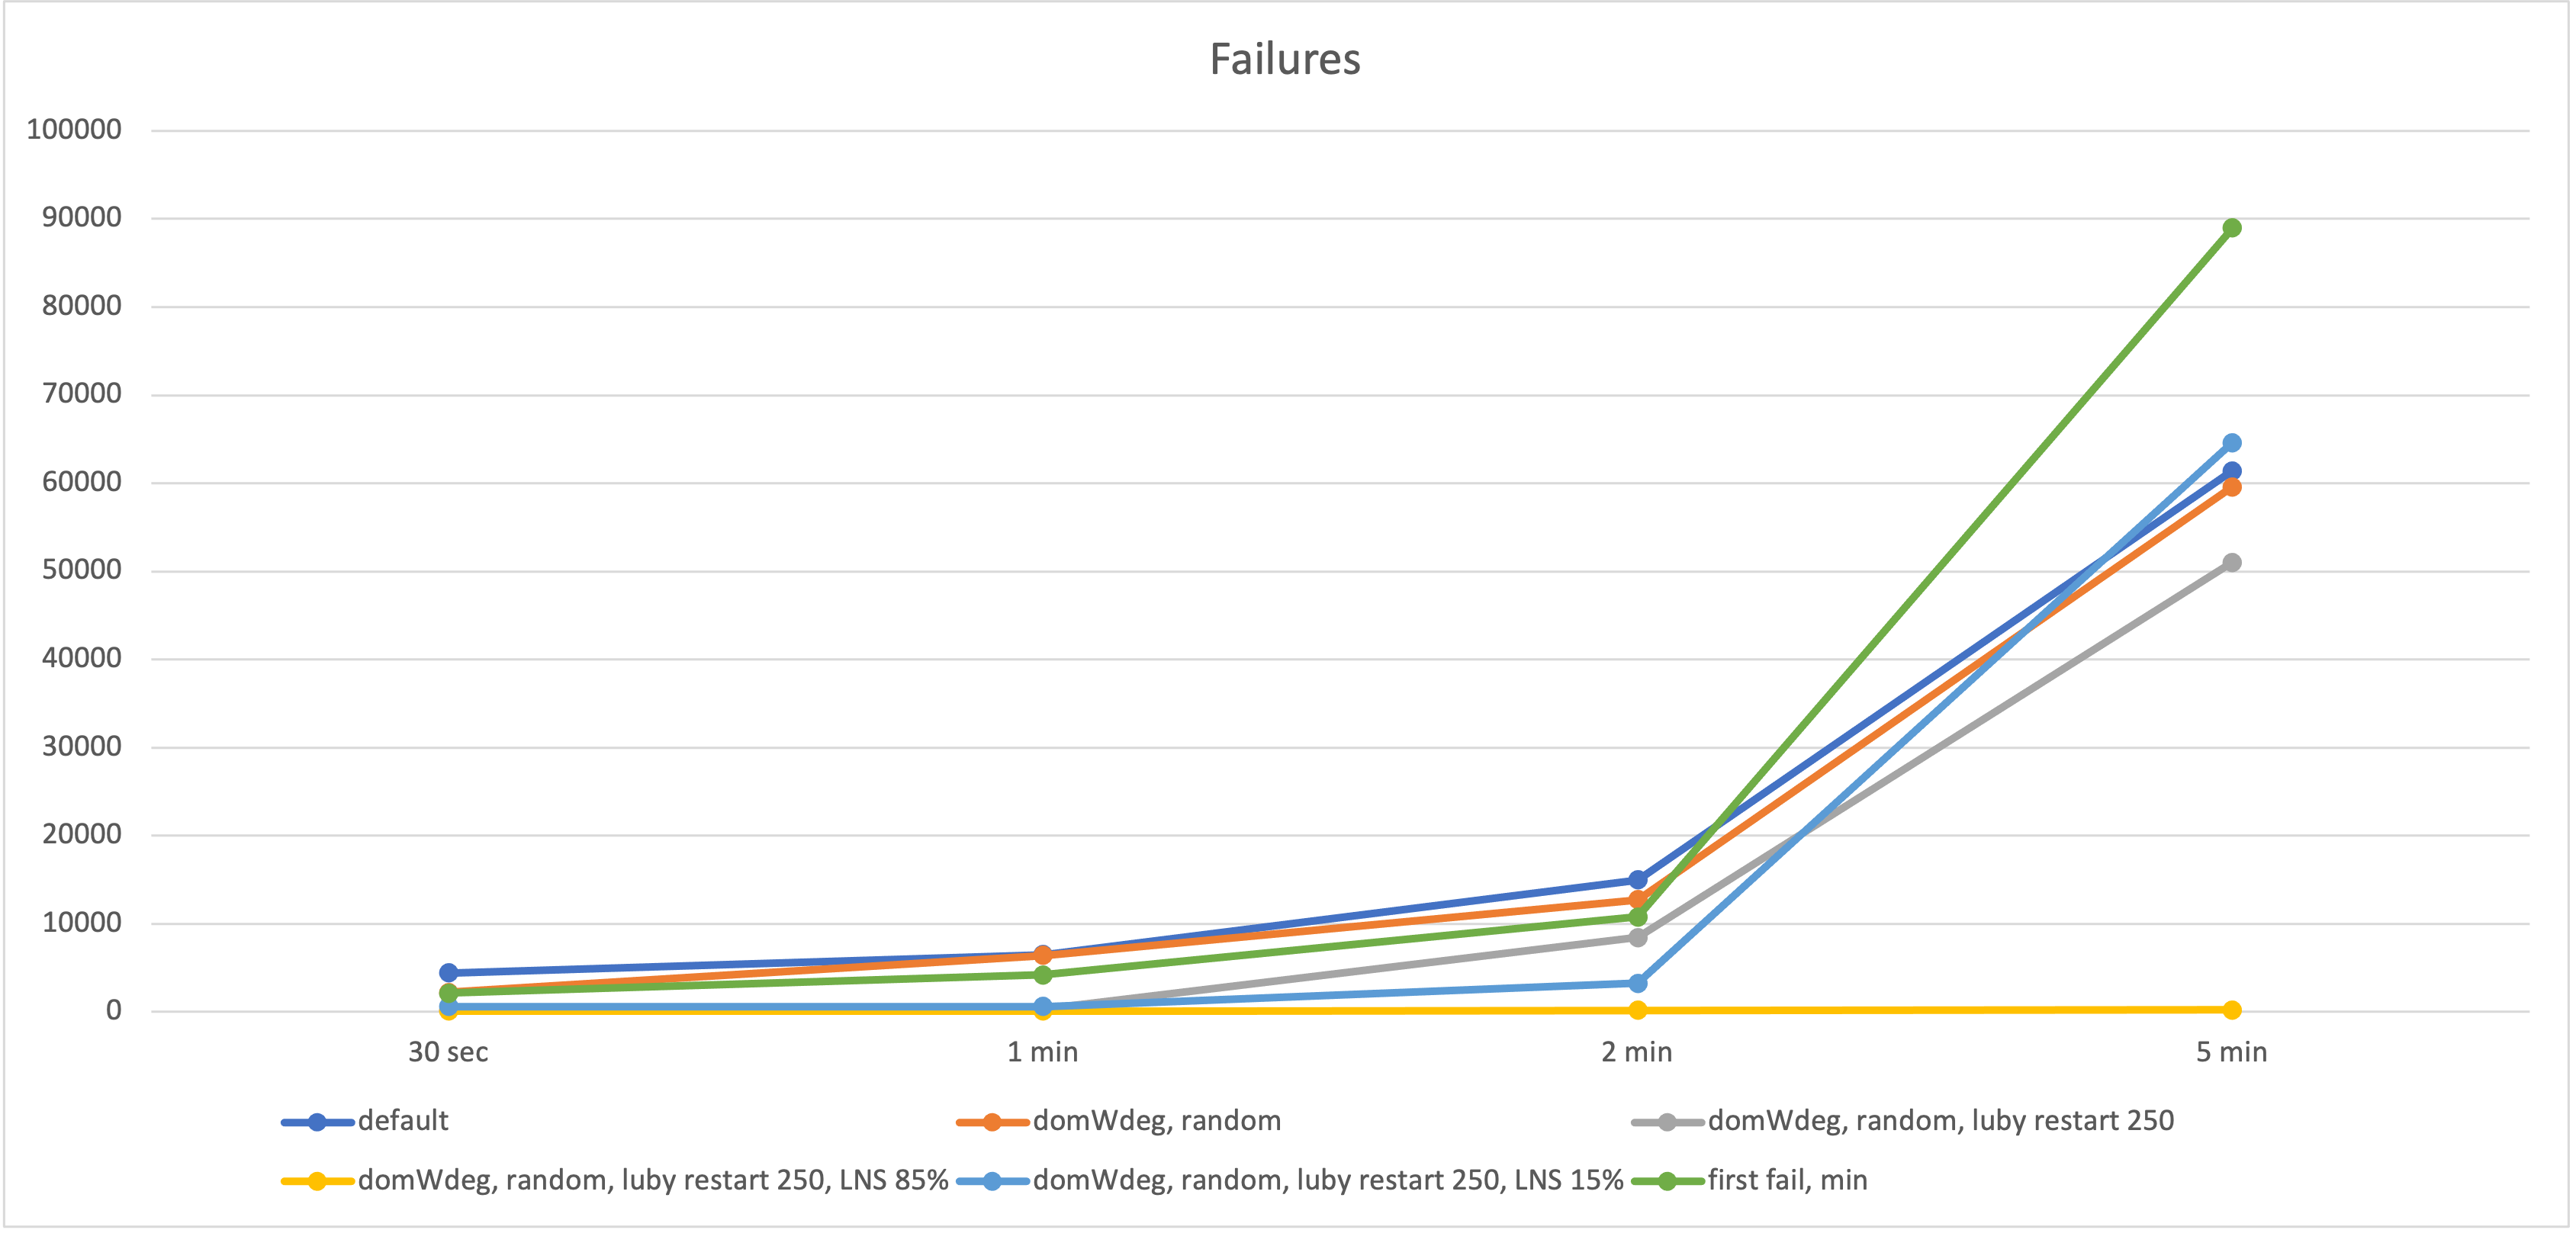
\includegraphics[width=0.8\columnwidth]{../graphs/pr03-failures.png}
    \caption{Failures graph for \textbf{pr03}.}
\end{figure}

{
\renewcommand{\arraystretch}{2}
\begin{longtable}[h]{| c | c | c | c | c |}
    \hline
    \textbf{Objective function} & \multicolumn{3}{c}{Time limit} & \\
    \hline
    \textbf{Search strategy} & \textbf{\textit{30 sec}} & \textbf{\textit{1 min}} & \textbf{\textit{2 min}} & \textbf{\textit{5 min}} \\
    \hline
    \endhead
    default search                                & 115.509.650 & 114.839.860 & 114.398.320 & 112.464.110 \\
    \hline
    domWdeg, random                               & 121.740.300 & 120.682.530 & 119.103.210 & 115.945.820 \\
    \hline
    \textit{domWdeg, random, Luby restart L=250}  & 117.949.620 & 115.131.230 & 107.202.080 & 106.628.240 \\
    \hline
    domWdeg, random, Luby restart L=250, LNS 85\% & 117.949.620 & 117.134.950 & 115.183.530 & 108.694.910 \\
    \hline
    domWdeg, random, Luby restart L=250, LNS 15\% & 119.136.170 & 119.121.920 & 117.696.110 & 116.622.700 \\
    \hline
\end{longtable}
}
\begin{figure}[H]
    \centering
    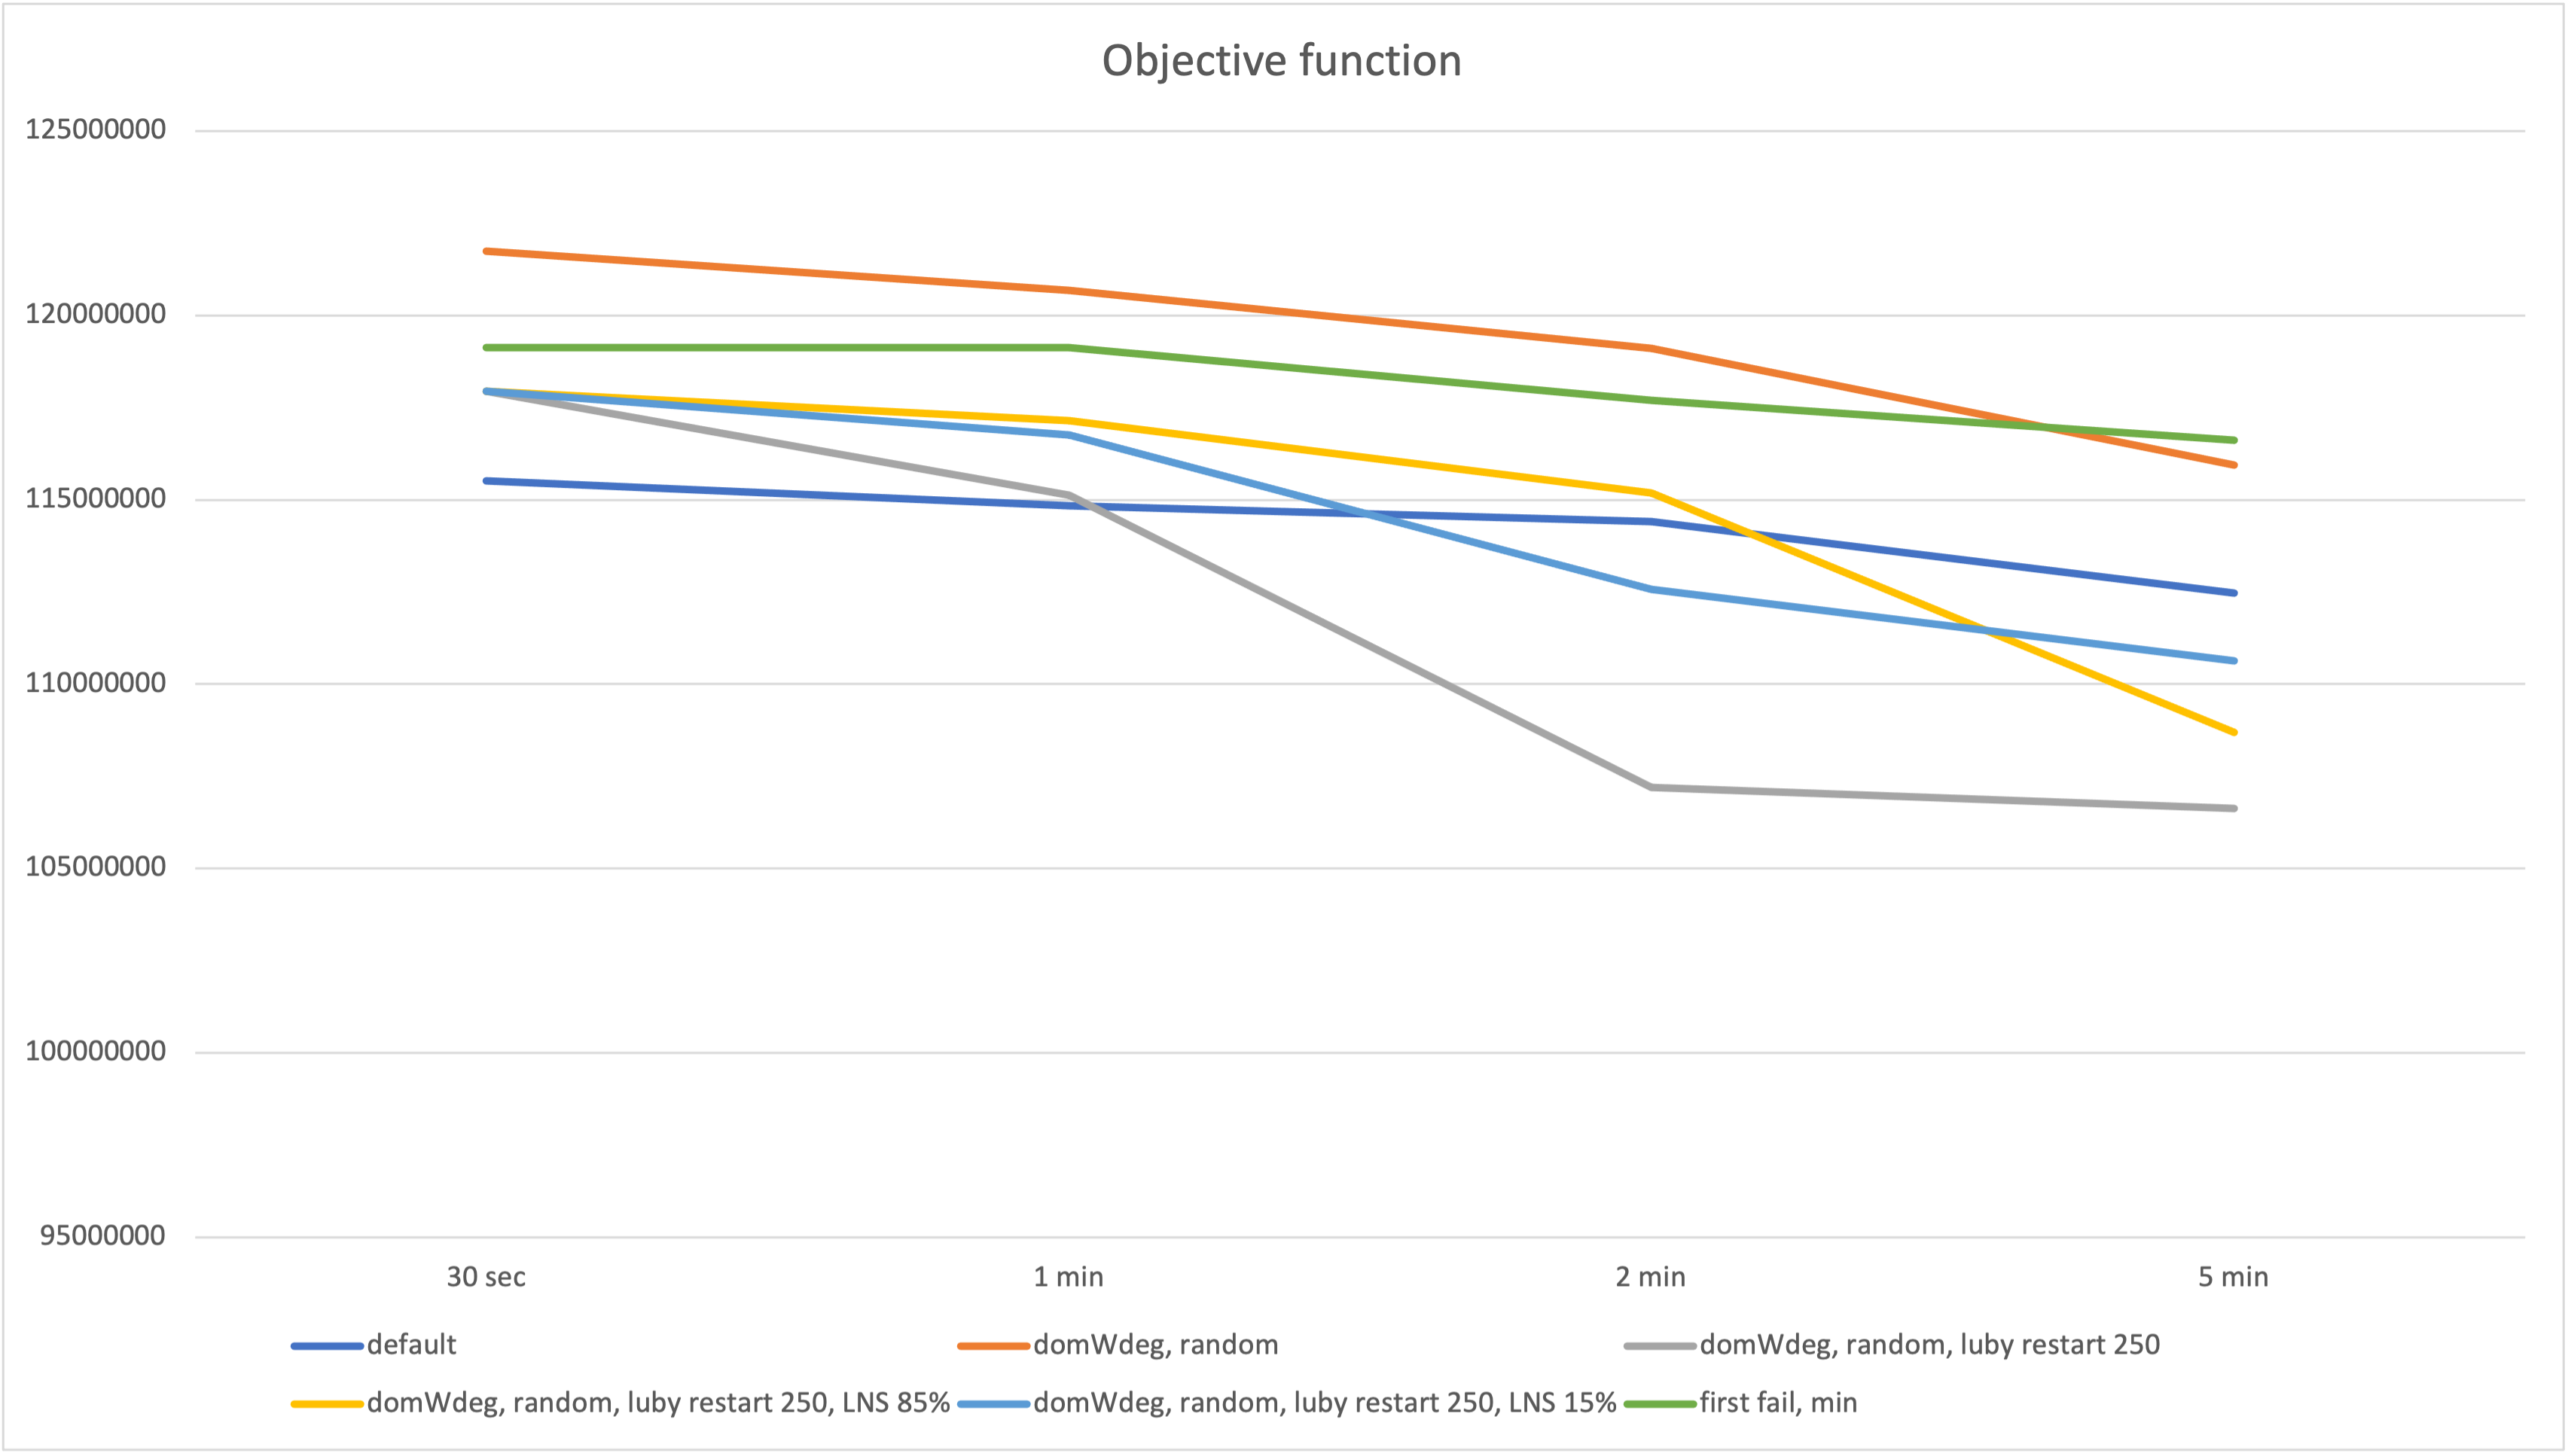
\includegraphics[width=0.8\columnwidth]{../graphs/pr03-objf.png}
    \caption{Objective functions graph for \textbf{pr03}.}
\end{figure}

{
\renewcommand{\arraystretch}{2}
\begin{longtable}[h]{| c | c | c | c |}
    \hline
    \textbf{Weights} & \textbf{Objective function} & \textbf{Total distance} & \textbf{Used vehicles} \\
    \hline
    \endhead
    $\alpha = 10, \beta = 0$ & 93.447.180 &  9.344.718 & 19 \\
    \hline
    $\alpha = 7, \beta = 3$  & 66.163.915 &  9.451.981 & 16 \\
    \hline
    $\alpha = 5, \beta = 5$  & 47.259.985 &  9.451.981 & 16 \\
    \hline
    $\alpha = 3, \beta = 7$  & 34.983.740 & 11.661.200 & 20 \\
    \hline
    $\alpha = 0, \beta = 10$ &        100 & 11.077.735 & 10 \\
    \hline
\end{longtable}
}
\begin{figure}[H]
    \centering
    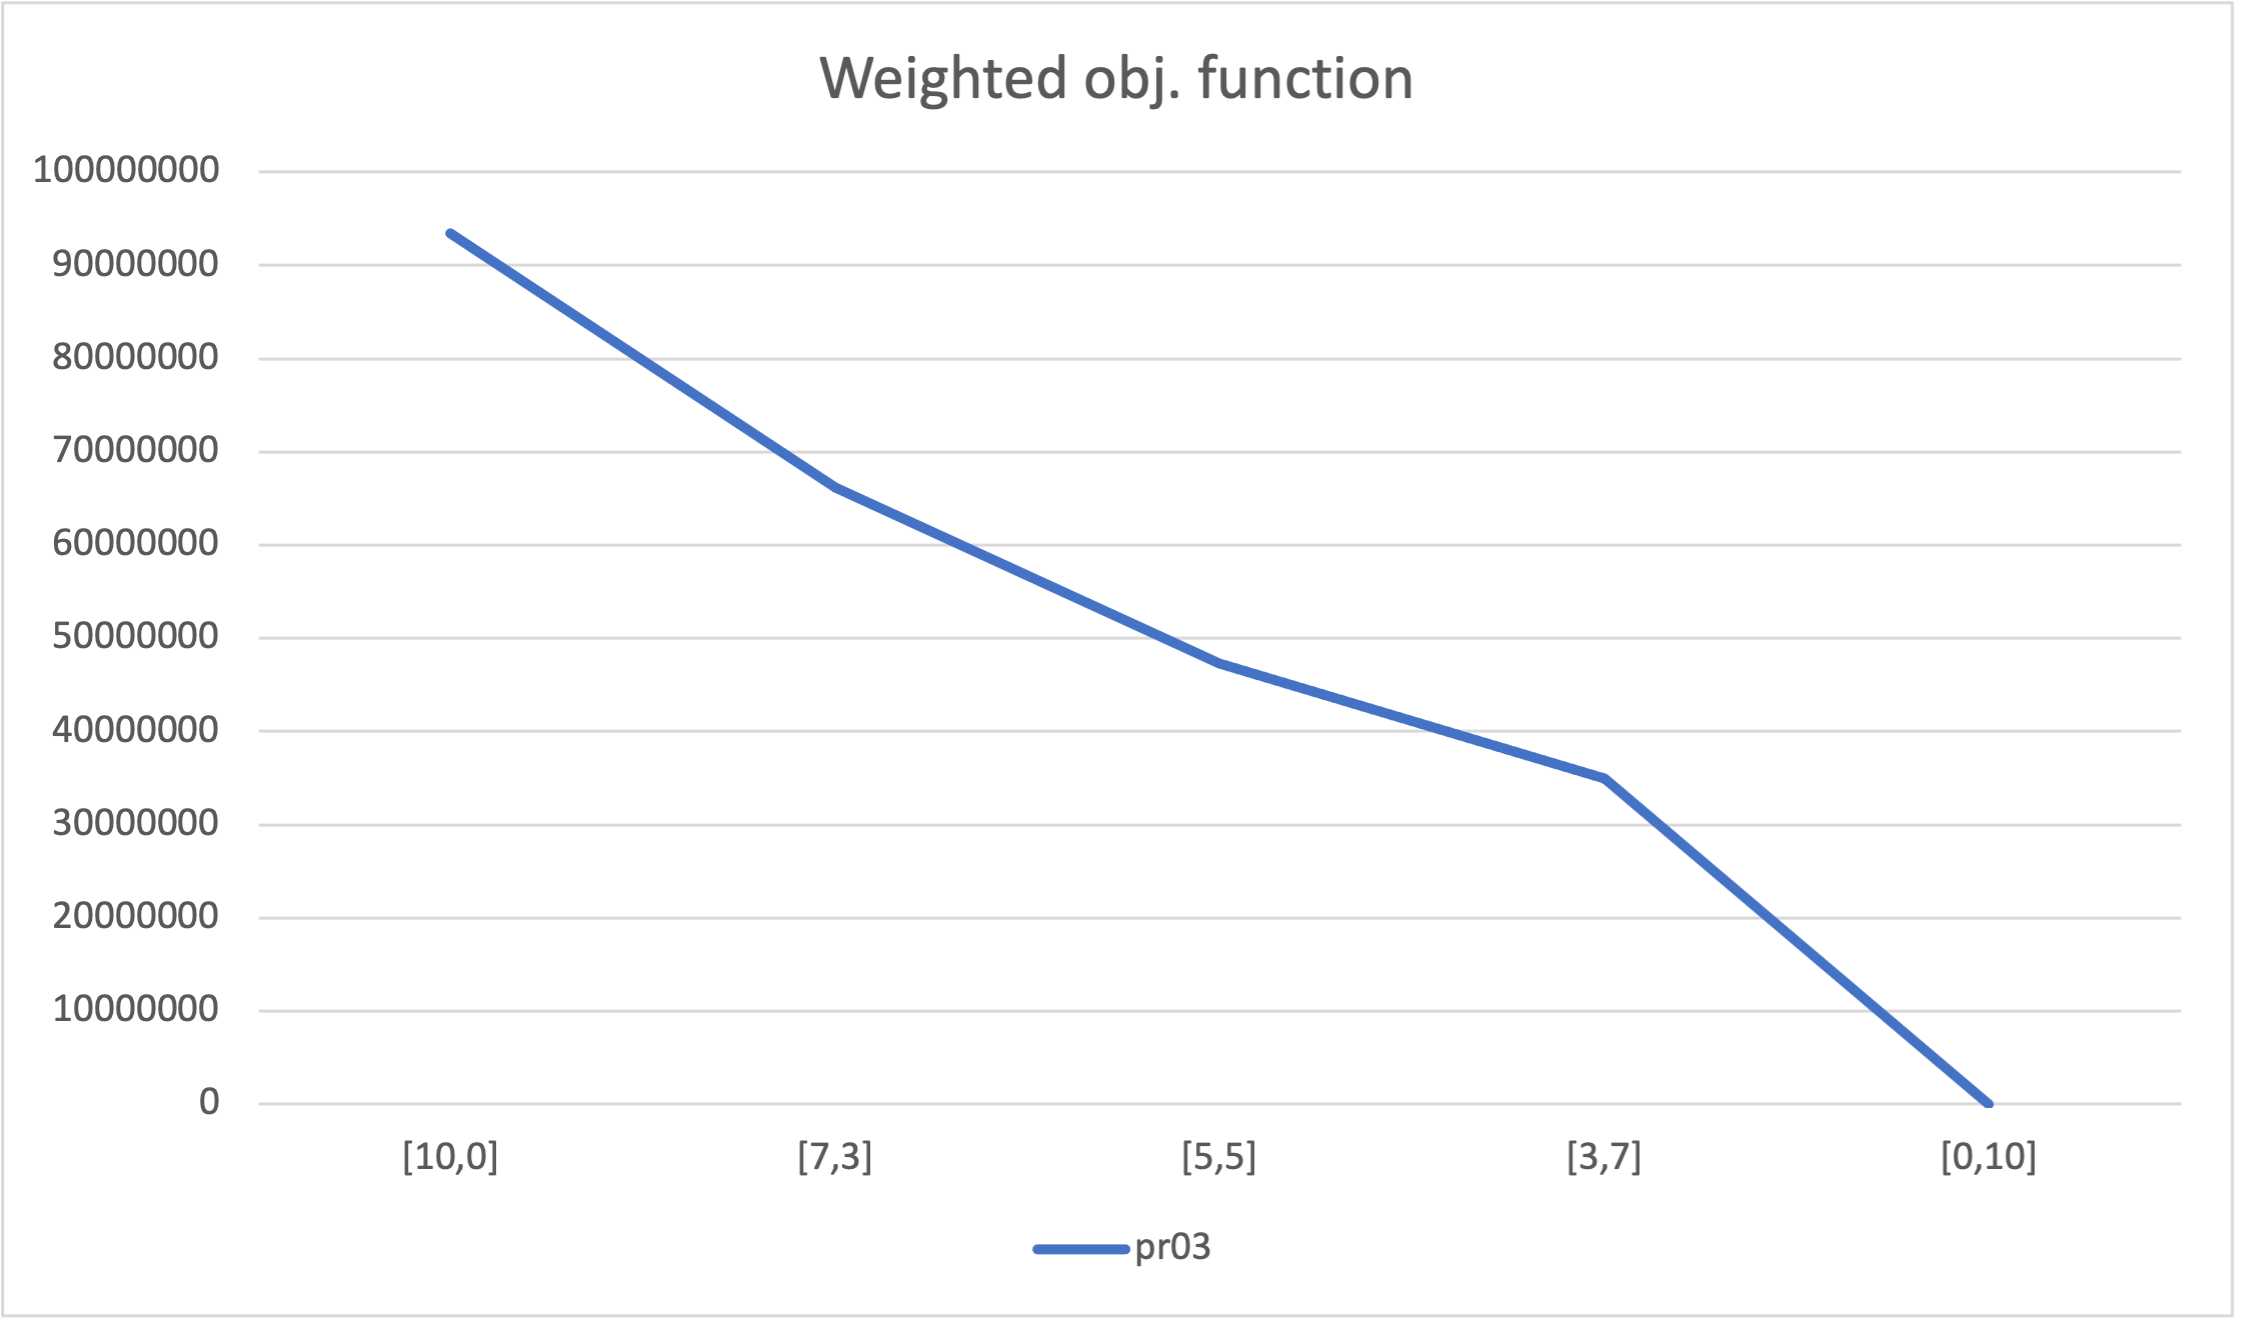
\includegraphics[height=0.25\textheight]{../graphs/pr03-wobjf.png}
    \caption{Weighted objective functions graph for \textbf{pr03}.}
\end{figure}

\begin{figure}[H]
    \centering
    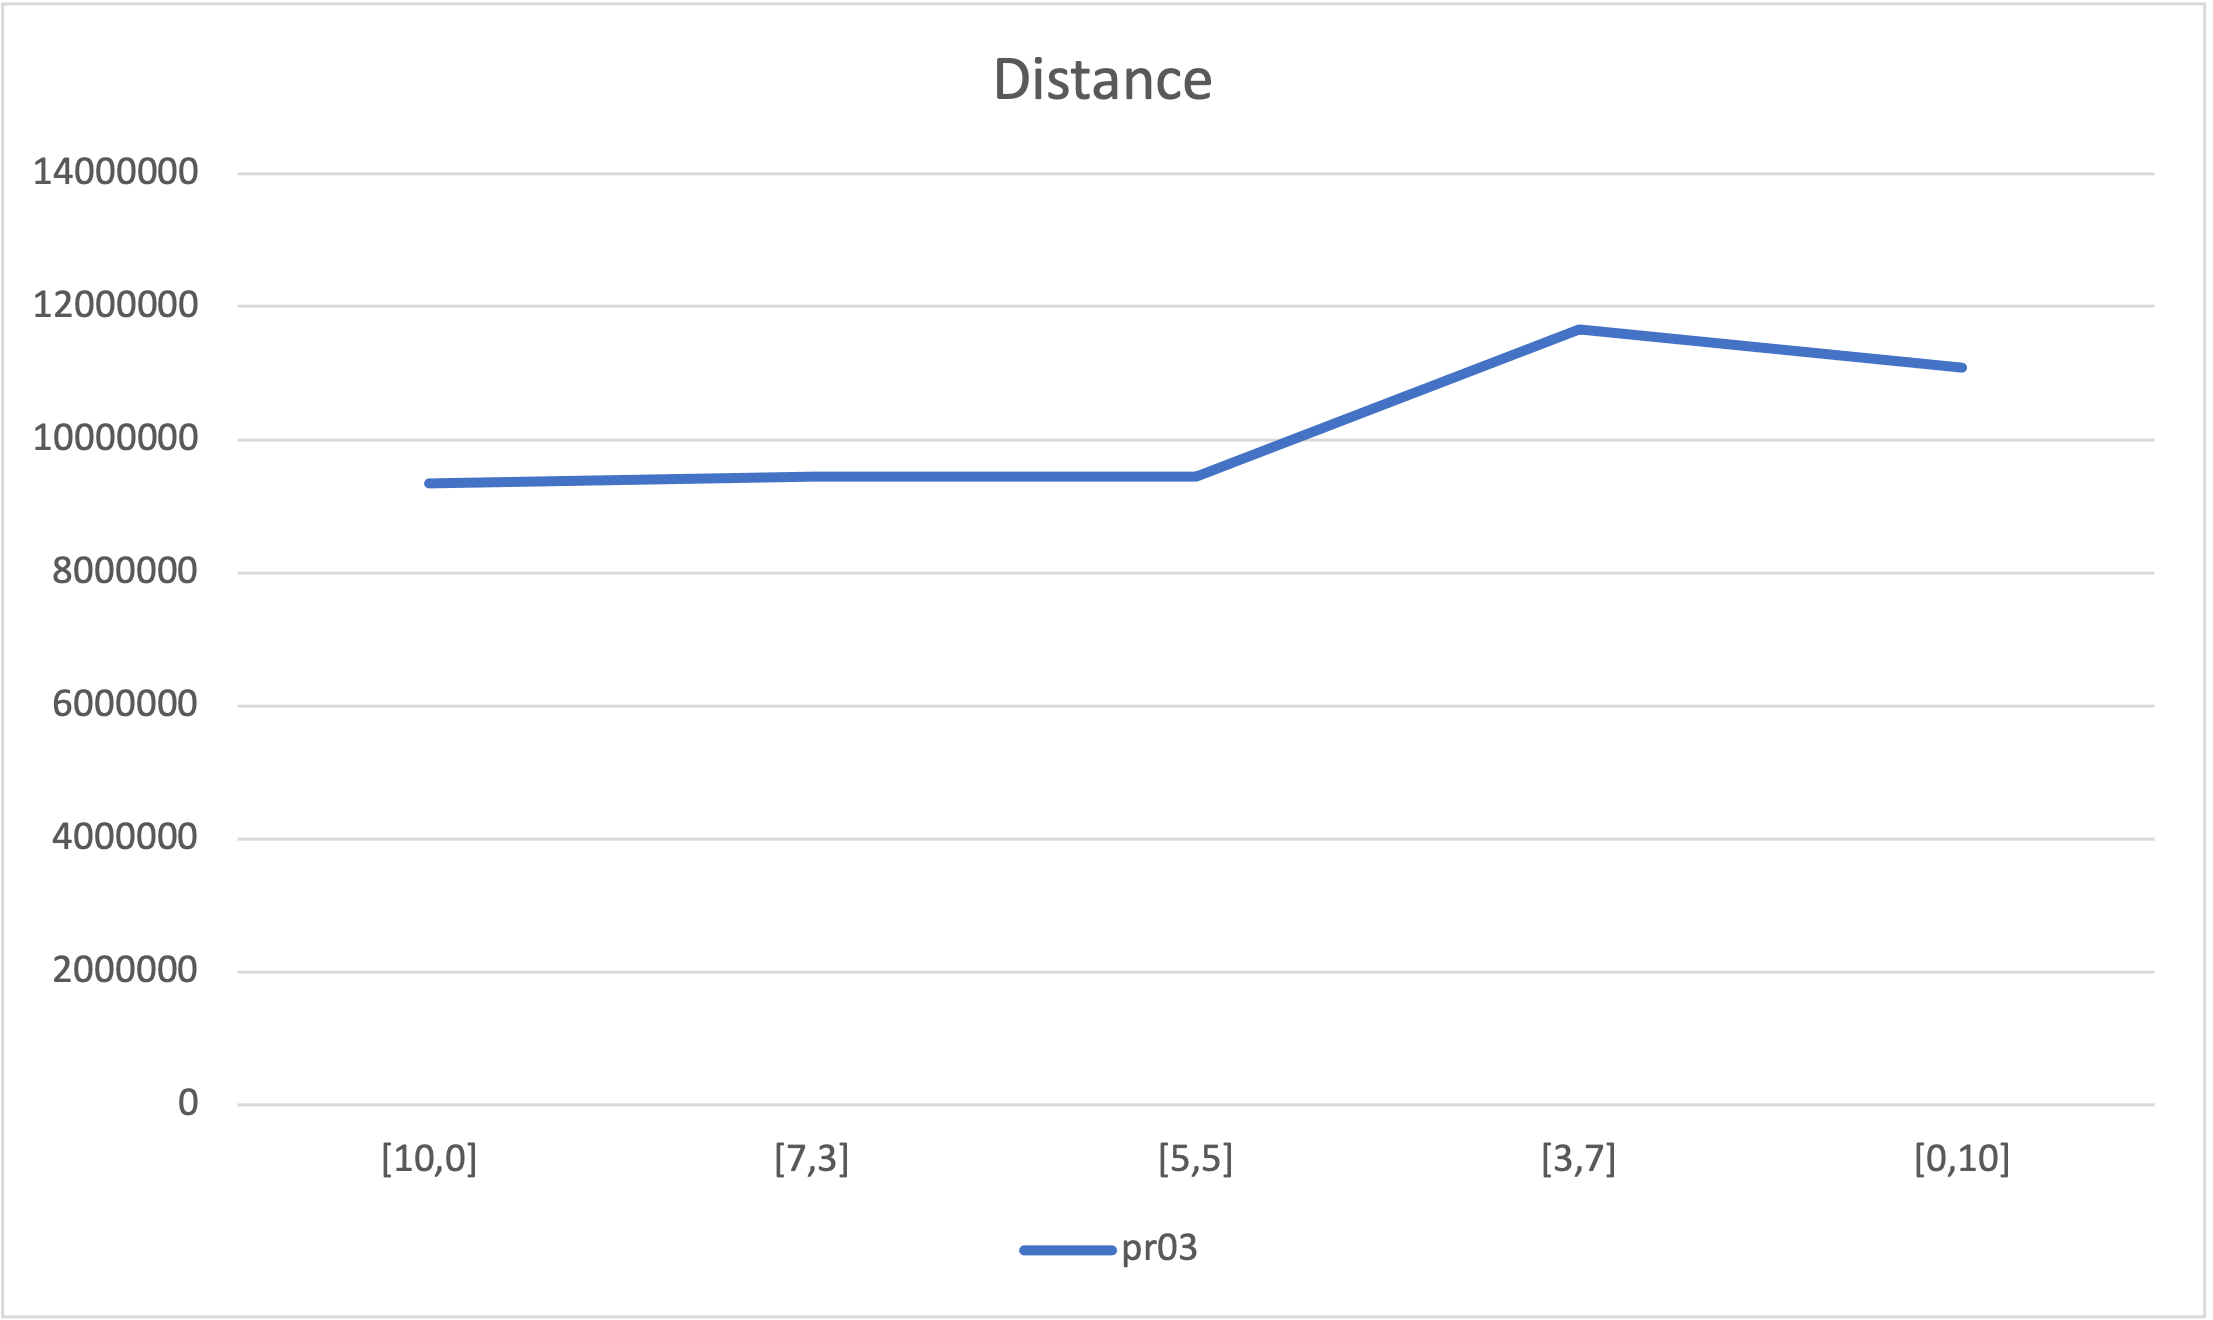
\includegraphics[height=0.25\textheight]{../graphs/pr03-distance.png}
    \caption{Distances graph for \textbf{pr03}.}
\end{figure}

\begin{figure}[H]
    \centering
    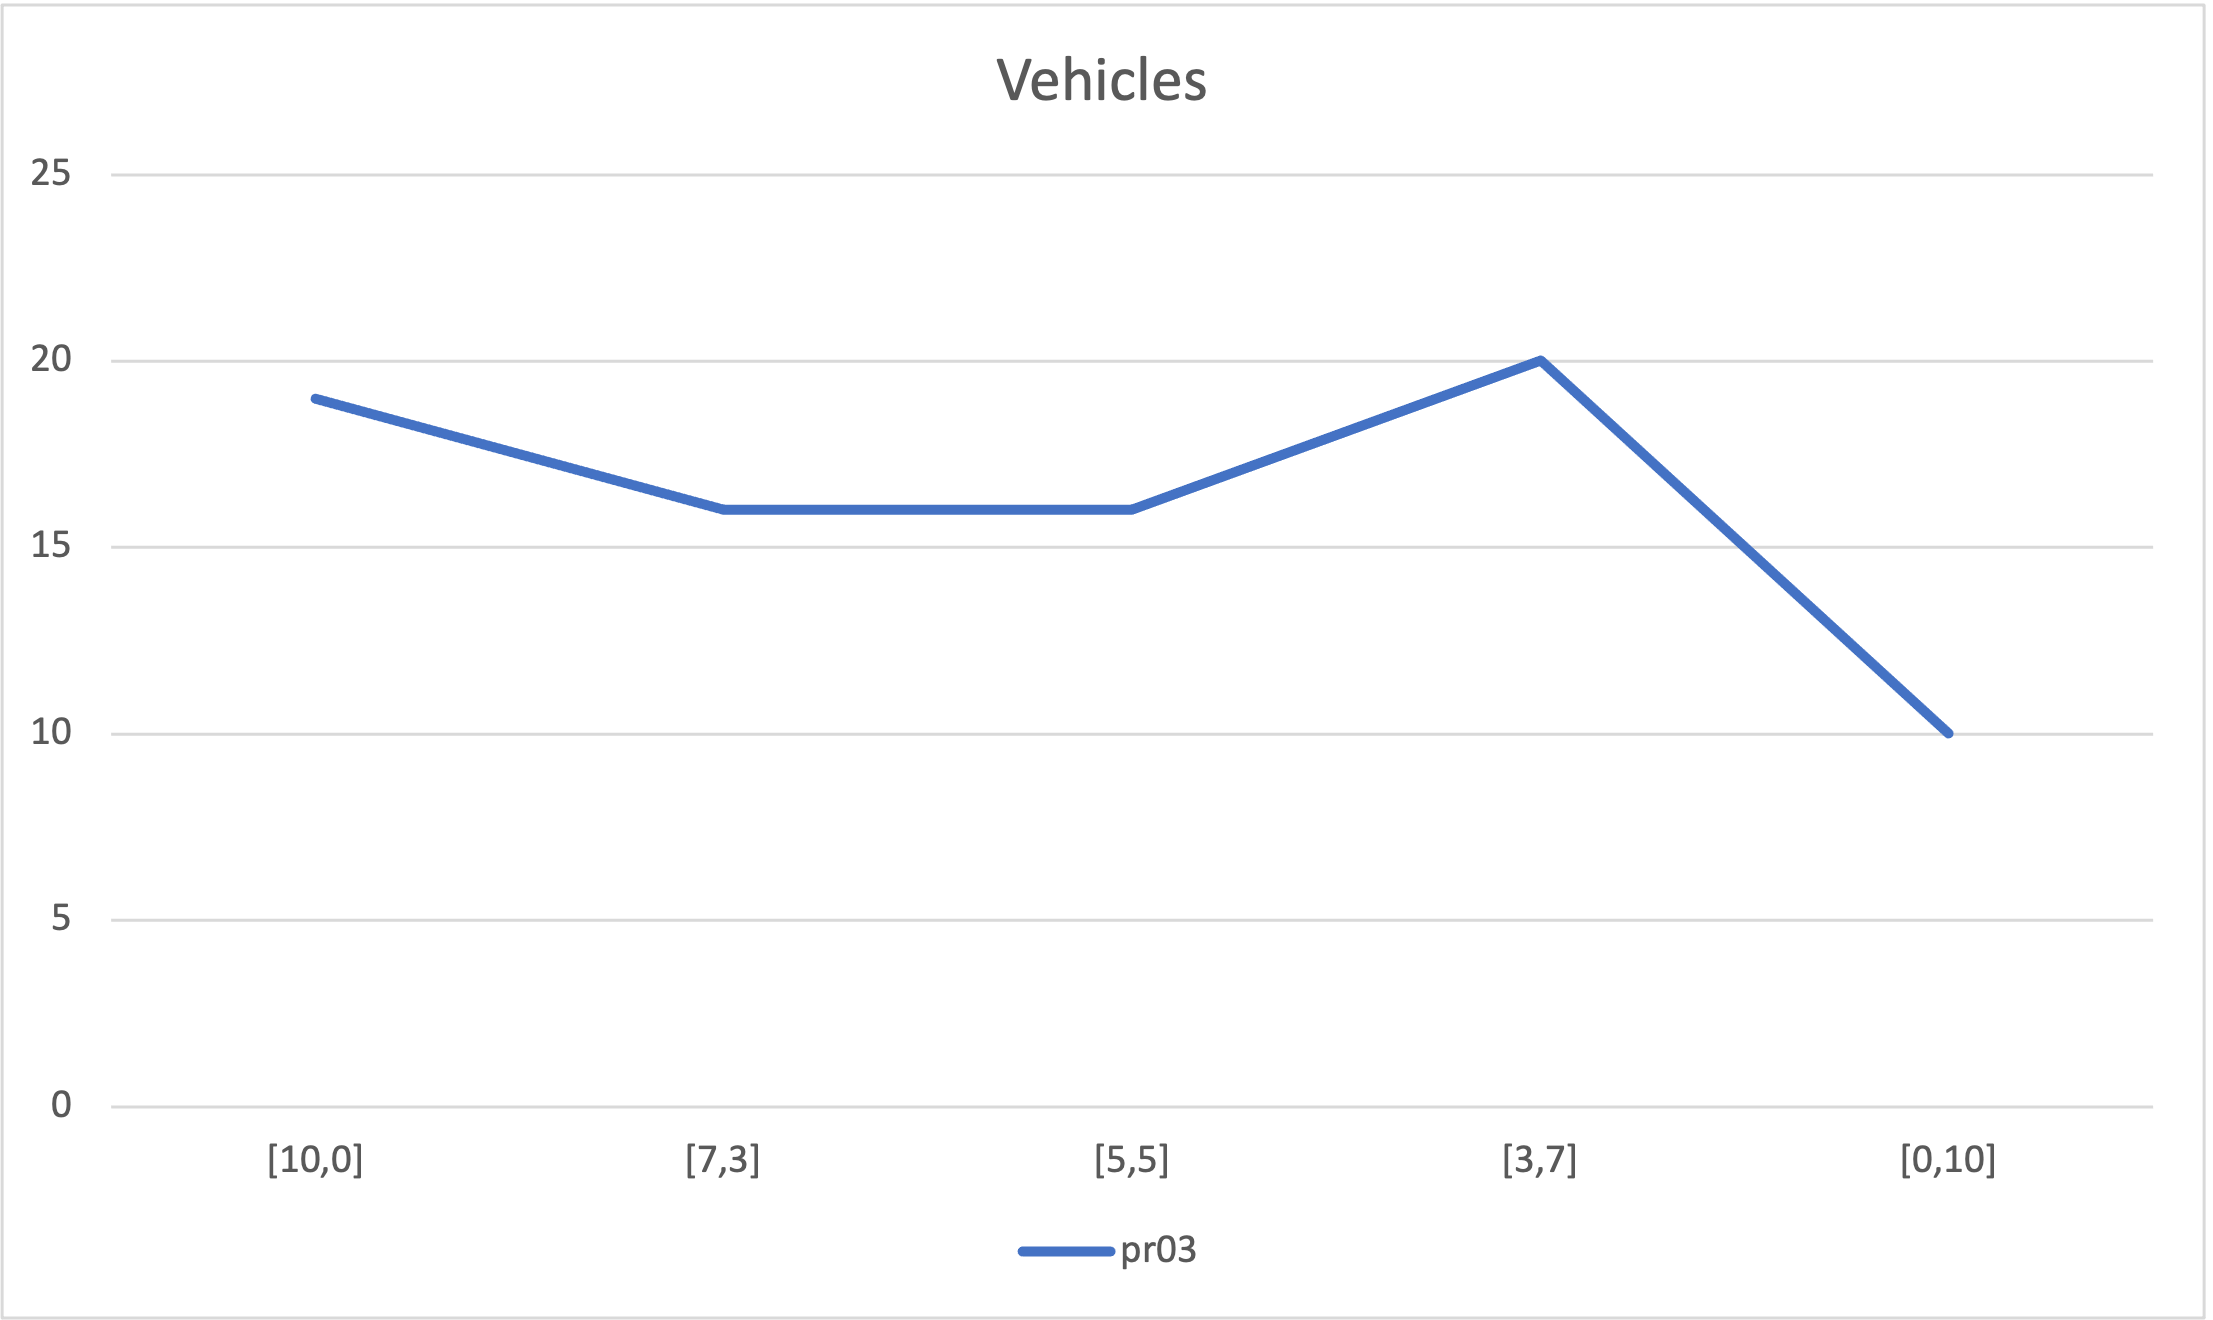
\includegraphics[height=0.25\textheight]{../graphs/pr03-vehicles.png}
    \caption{Vehicles used graph for \textbf{pr03}.}
\end{figure}

\newpage